% Section 4: Discussion, Comparison with k-NN, and Python (Slides 30-32)

% Slide 30: Discussion of Decision Trees
\begin{frame}{بحث و ارزیابی درخت‌های تصمیم}{\lr{Discussion of Decision Trees}}
  \begin{columns}[T]
    \begin{column}{0.48\textwidth}
      \begin{block}{مزایای کلیدی (\lr{Advantages})}
        \begin{itemize}
          \setlength{\itemsep}{3pt}
          \item \textbf{هزینه کم ساخت:} الگوریتم سریع و محاسبات سبک
          \item \textbf{سرعت بسیار بالا در تست:} طبقه‌بندی آنی رکوردهای جدید
          \item \textbf{تفسیرپذیری شفاف:} ساختار شفاف و قابل فهم (\lr{White-box})
          \item \textbf{بی‌نیازی از مقیاس‌بندی:} عدم نیاز به نرمال‌سازی داده‌ها
          \item \textbf{مقاومت در برابر ویژگی‌های هرز:} عدم تأثیرپذیری از ویژگی‌های نامرتبط
        \end{itemize}
      \end{block}
    \end{column}
    \begin{column}{0.48\textwidth}
      \begin{alertblock}{محدودیت‌ها و معایب (\lr{Disadvantages})}
        \begin{itemize}
          \setlength{\itemsep}{3pt}
          \item \textbf{مرزهای موازی محورها:} تقریب پلکانی نامناسب برای مرزهای تصمیم مورب یا غیرخطی پیچیده
          \item \textbf{ناپایداری و واریانس بالا:} تغییرات جزئی در داده‌های آموزش می‌تواند ساختار کل درخت را دگرگون کند.
          \item \textbf{آسیب‌پذیری در برابر نویز:} تمایل شدید به بیش‌برازش (\lr{Overfitting}) در صورت رشد آزادانه
        \end{itemize}
      \end{alertblock}
    \end{column}
  \end{columns}
\end{frame}

% Slide 31: Comparing Decision Trees and k-NN
\begin{frame}{مقایسه درخت‌های تصمیم و الگوریتم \lr{k-NN}}{\lr{Comparing Decision Trees and k-NN}}
  \centering\small
  \resizebox{\textwidth}{!}{%
  \begin{tabular}{|l|p{5.5cm}|p{5.5cm}|}
    \hline
    \textbf{معیار مقایسه} & \textbf{درخت تصمیم (\lr{Decision Tree})} & \textbf{نزدیک‌ترین همسایگی (\lr{k-NN})} \\
    \hline
    \textbf{نوع رویکرد یادگیری} & مشتاق (\lr{Eager}) -- ساخت مدل صریح سراسری & تنبل (\lr{Lazy}) -- عدم ساخت مدل تا زمان آزمون \\
    \hline
    \textbf{شکل مرزهای تصمیم} & خطوط متعامد و موازی با محورها (\lr{Axis-parallel}) & مرزهای دلخواه، پیوسته و منعطف (\lr{Arbitrary}) \\
    \hline
    \textbf{هزینه محاسباتی تست} & بسیار سریع و سبک: $O(\text{depth})$ & سنگین و وابسته به کل داده‌ها: $O(N \cdot D)$ \\
    \hline
    \textbf{تفسیرپذیری} & بسیار بالا؛ قابل فهم و نمایش در قالب درخت & پایین؛ جعبه سیاه مبتنی بر فاصله \\
    \hline
    \textbf{حساسیت به مقیاس} & کاملاً نامتغیر در برابر تغییر مقیاس ویژگی‌ها & بسیار حساس به نرمال‌سازی و مقیاس متغیرها \\
    \hline
    \textbf{ویژگی‌های نامرتبط} & مقاومت بالا با نادیده گرفتن در شاخه‌ها & افت شدید دقت به دلیل لعنت ابعاد \\
    \hline
  \end{tabular}%
  }
\end{frame}

% Slide 32: Tree Induction in Python
\begin{frame}{القای درخت تصمیم در پایتون}{\lr{Tree Induction in Python (scikit-learn)}}
  \begin{latin}
  \begin{center}
    \fcolorbox{codeborder}{codebg}{
      \begin{minipage}{0.96\textwidth}
        \ttfamily\footnotesize
        \textbf{from} sklearn.tree \textbf{import} DecisionTreeClassifier, plot\_tree\\[2pt]
        \textcolor{gray}{\# Train classifier}\\
        dt\_learner = DecisionTreeClassifier(criterion=\textcolor{teal}{'gini'}, max\_depth=10)\\
        dt\_learner.fit(preprocessed\_training\_data, training\_labels)\\[2pt]
        \textcolor{gray}{\# Use classifier to predict labels}\\
        prediction = dt\_learner.predict(preprocessed\_unseen\_data)\\[2pt]
        \textcolor{gray}{\# Plot the decision tree}\\
        plot\_tree(dt\_learner)
      \end{minipage}
    }
  \end{center}
  \end{latin}
  \vspace{-0.1cm}
  \begin{center}
    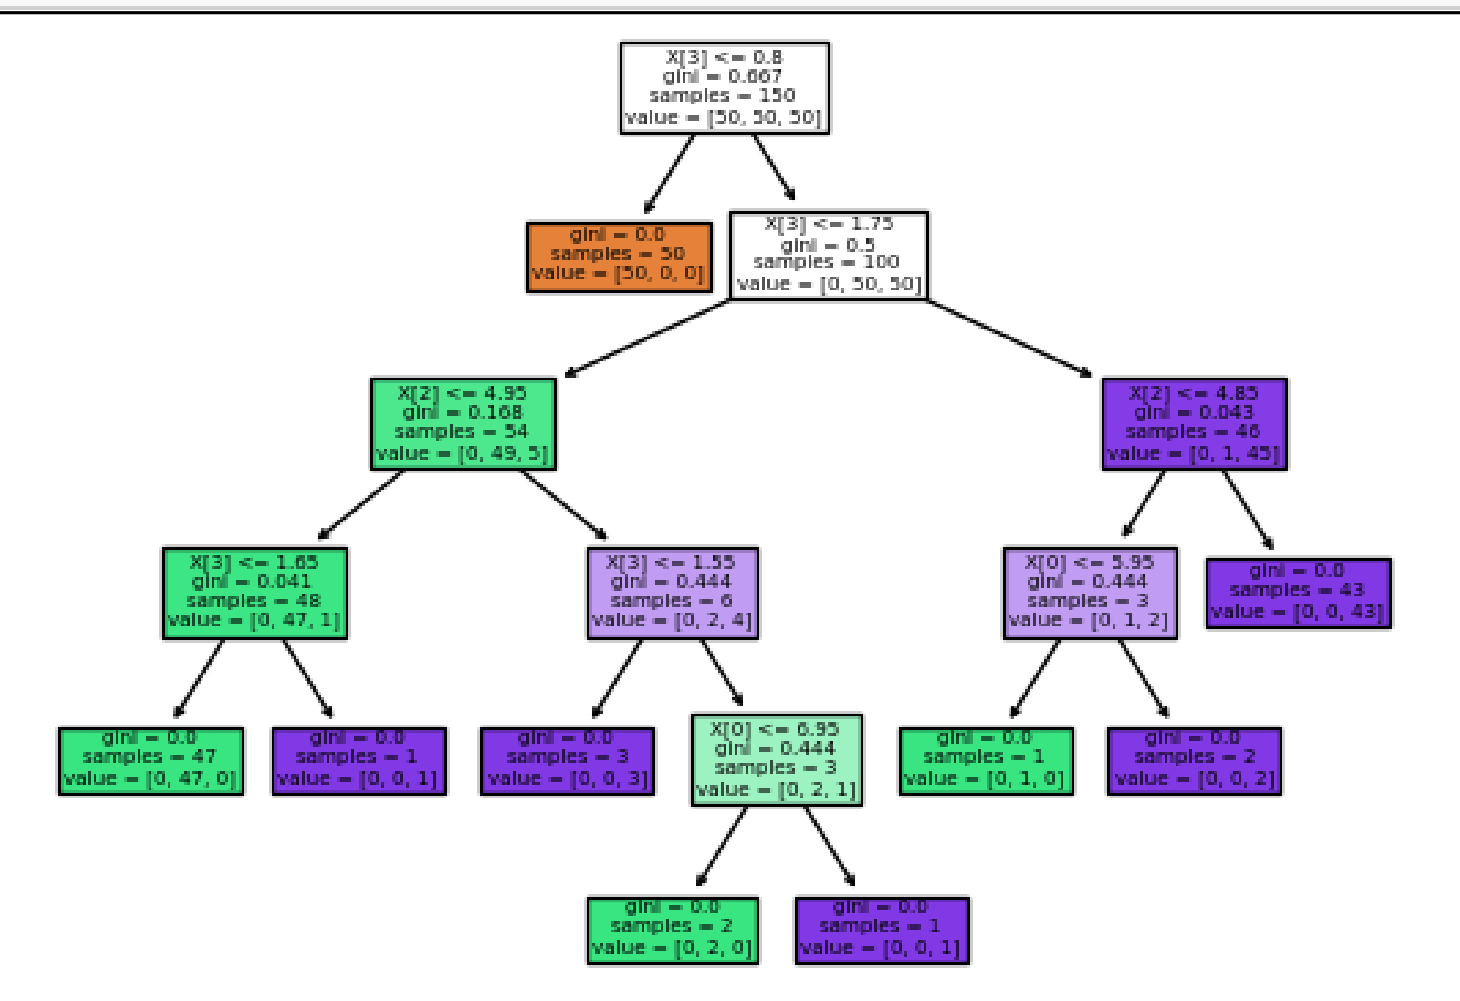
\includegraphics[width=0.70\textwidth,height=3.4cm,keepaspectratio]{images/slide32_tree_plot.png}
  \end{center}
\end{frame}
